\section{Understanding the fluctuations}
We have  looked at the waveform  fluctutations because it is  a way to
check the  detector's simulation. But it  is also important  to get an
idea of  the detector  sensitivity. There is  the formula given  for a
square law detector:
\begin{equation}
  F = \frac{k_{B} T_{sys}}{\sqrt{\Delta B \tau}}
  \label{eq:sensitivity}
\end{equation}
This formula  is in fact the  ratio of the  RMS of a square  law radio
detector and an integration term (similar to a $\sqrt{N}$).  It states
that the  minimum observable signal  (or the detector  sensitivity) is
the   system  noise   temperature  reduced   by  how   much   you  can
integrate/average it. In  reality it is a good figure  of merit but it
is    not   completely    correct    for   all    the   cases.     The
equation~\ref{eq:sensitivity} is only  correct when the integration is
done  by a numerical  filter with  the frequency  $\frac{1}{\tau}$. We
want to understand better this formula, several cases are discussed in
the following paragraphs.


\subsection{case study}
\paragraph{derivation of the equation}
The  derivation of  the formula~\ref{eq:sensitivity}  is given  in the
book    "Tools   of    Radio   Astronomy"    (T.L~Wilson,   K.~Rohlfs,
S.~Huttemeister).  One wants  to find  the what  is the  value  of the
detectable  signal,  so we  look  at  the  standard deviation  of  the
recorded signal. The main steps are the following:
\begin{itemize}
\item take a radio detector with a bandwidth B, the amplitude of the signal $v(t)$ follows a gaussian distribution.
\item the signal goes through a square law detector $y = av(t)^2$. One
  can  compute the  mean  and  standard deviation  and  finds: $<y>  =
  a\sigma_v^2$ and $\sigma_y = \sqrt{2}a\sigma_v^2$ (with $<v^2> = <power> =
  kT_{sys}     G    B$).    (this     webpage    might     also    help:
  http://mathworld.wolfram.com/GaussianIntegral.html)
\item So we have: $\sigma_y = \sqrt{2} <y> $ , with $\sigma_y = k_B \Delta
  T G B$ so $\Delta T = \sqrt{2} T_{sys}$
\item now  if we  average over  a time $\tau$,  that means  we average
  over$ N = f_{Nyquist}*\tau$ points where $f_{Nyquist} = 2B$, and we reduce the fluctuation by a factor $\sqrt{N}$
\item we finally obtain: $\Delta T = \frac{T_{sys}}{\sqrt{B\tau}}$
\end{itemize}

So to  sum up, for  a input gaussian  signal followed by a  square law
detector we expect the  ratio $\rm \frac{\sigma}{\mu} = \sqrt{2}$. And
this  ratio  is then  modified  by  the  later processing,  averaging,
filtering.

\paragraph{ideal case}
Let's take the simple  case of a square law detector with
a bandwidth of  [0 - 2GHz] for instance.  We  produce a noise waveform
with a flat spectrum and look  at the distribution of the power in the
figure~\ref{fig:noise}.
\begin{figure}[!ht]
  \centering
  \hspace*{-3ex}
  \subfigure{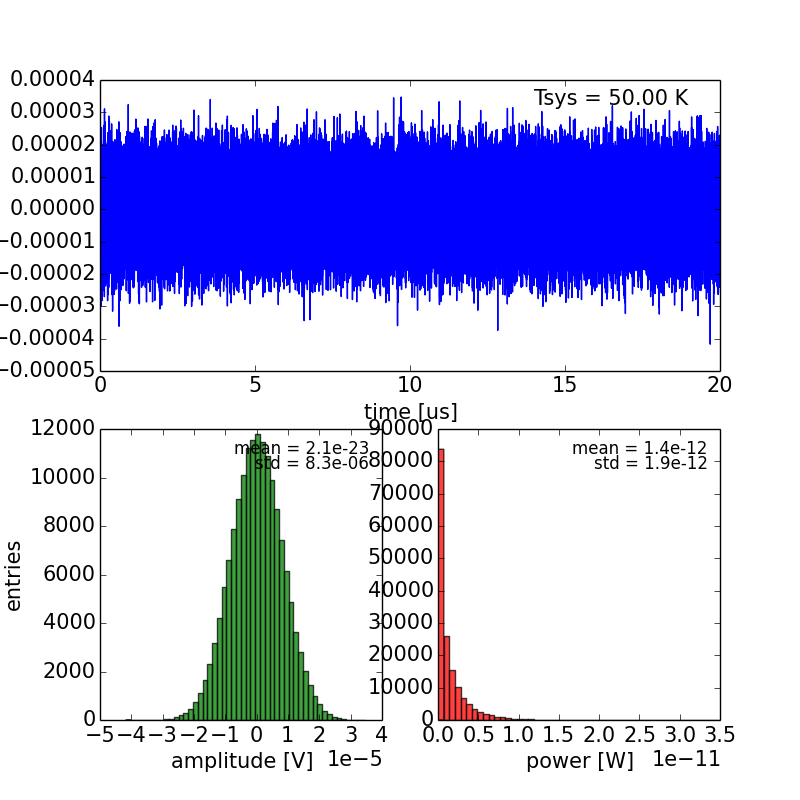
\includegraphics[width=0.60\linewidth]{noise.png}}
  \caption{}
  \label{fig:noise}
\end{figure}
We  can check that  the ratio  $\rm \frac{\sigma}{\mu}  $ is  equal to
$\sqrt{2}$.   Now if we  average with  a numerical  filter with  a cut
frequency  $f_{cut} =  1/\tau$ we  see  that it  follows the  expected
equation on the figure~\ref{fig:ratiofilter}. 
\begin{figure}[!ht]
  \centering
  \hspace*{-3ex}
  \subfigure{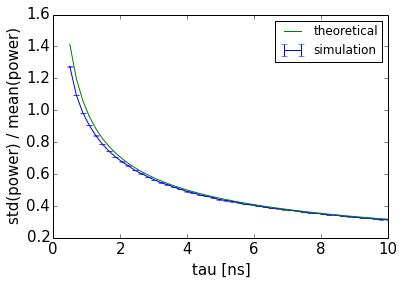
\includegraphics[width=0.60\linewidth]{rationumfilter.png}}
  \caption{}
  \label{fig:ratiofilter}
\end{figure}

\paragraph{bandwidth effect}
Now  we can  also look  at the  changes on  the fluctuations  when the
bandwidth  is  reduced.   Figure~\ref{fig:bw}  (left) shows  the  $\rm
\frac{\sigma}{\mu} $ ratio when we  keep the maximum frequency to 2GHz
but we reduce the lower bound  to reduce the bandwidth. The ratio stay
$\sqrt{2}$.   But  when we  filter,  we  see  discrepancy between  the
expected  ratio   and  the  simulated   one  (see  figure~\ref{fig:bw}
(right)). We see  that if we reduce the bandwidth,  the ratio is lower
than  expected and  plateaus at  for the  high frequency  filters (low
$\tau$) but  matches the  formulas at the  low frequency  filter (high
$\tau$).  This can be understood when we think about the FFTs (or look
at them  on figure~\ref{fig:fft}). The fourier transform  of the power
for  a signal  at frequencies  between [f1  - f2]  has  a contribution
between [0 ;  $\Delta B/2$] and another one between  [2*f1 ; 2*f2]. On
the  figure we  see  an example  for an  input  spectrum of  [1.5 ;  2
  GHz]. If we  filter with a frequency $f_{cut}  $smaller than $\Delta
B/2$ we follow the equation because we have a full bandwidth from [0 ;
  $f_{cut}$], if $f_{cut}$  is larger then we go into  the hole in the
power spectrum and  we don't add any frequency  in the average, that's
why the ratio goes to a constant.

\begin{figure}[!ht]
  \centering
  \hspace*{-3ex}
  \subfigure{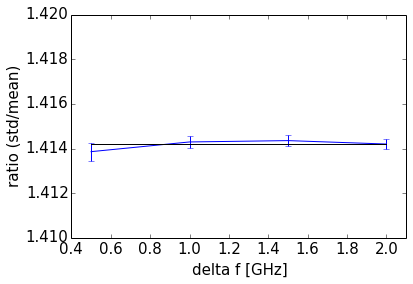
\includegraphics[width=0.45\linewidth]{ratiodiffBW.png}}
  \subfigure{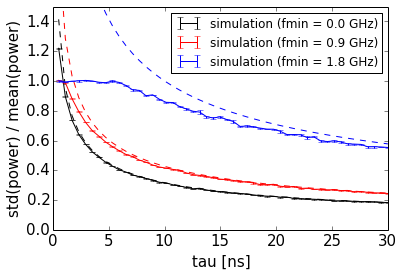
\includegraphics[width=0.45\linewidth]{rationumfilterdiffBW.png}}
  \caption{left: ratio $\frac{\sigma}{\mu}$ versus the lower frequency
    $f_min$ of the noise spectrum. rigt: the ratio when we apply a low
    pass filter of frequency cut $f_{cut}= 1/\tau$ to the power. It is
    shown for three different $f_{min}$}
  \label{fig:bw}
\end{figure}

\begin{figure}[!ht]
  \centering
  \hspace*{-3ex}
  \subfigure{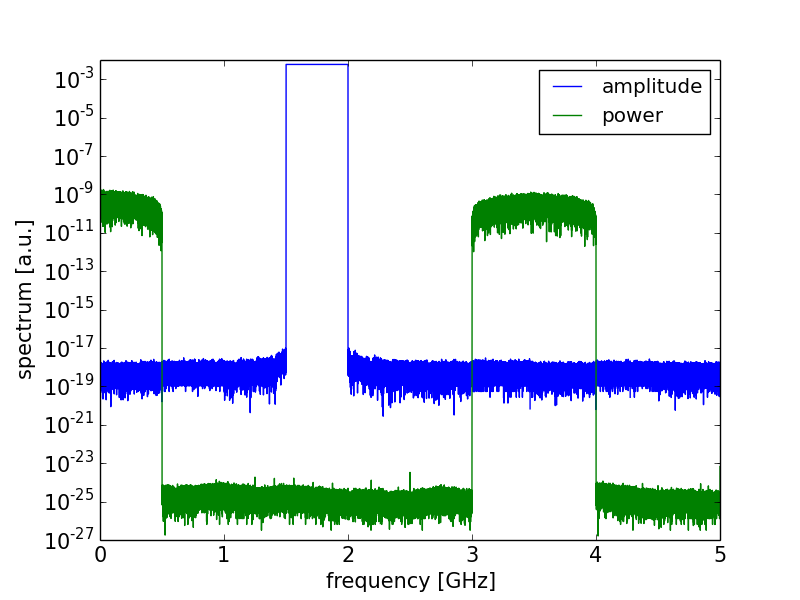
\includegraphics[width=0.60\linewidth]{specnoise.png}}
  \caption{example of spectra of the  amplitude and power for an input
    noise signal. We see the two contribution in the spectrum of the power, and the hole if $\Delta B/2 \leq f_{min}$}
  \label{fig:fft}
\end{figure}


\paragraph{sliding window}
If instead of  filtering by cutting the frequency  spectrum we average
over  several bins,  i.e. a  sliding window  average.  If  we consider
$\tau$ as  the window size we  see (fig~\ref{fig:slidingwindow}) that
the ratio  doesn't follow the equation~\ref{sensitivity}.  There is an
additional factor  to be  added.  This shows  that the  formula really
depends on the processing, and one  should use it as a figure of merit
or a rough estimation.
\begin{figure}[!ht]
  \centering
  \hspace*{-3ex}
  \subfigure{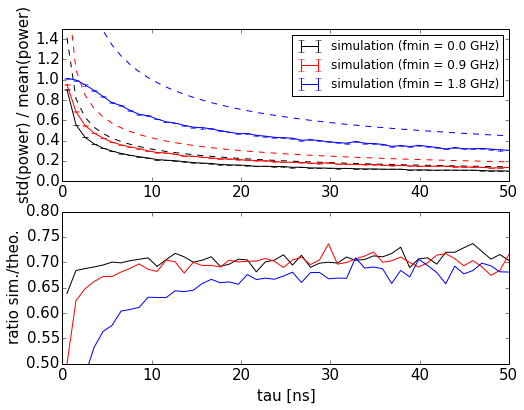
\includegraphics[width=0.60\linewidth]{slidingwindow.png}}
  \caption{$\frac{\sigma}{\mu}$ ratio after  applying a sliding window
    of size $\tau$ for different $f_{min}$}
  \label{fig:slidingwidow}
\end{figure}
